\documentclass[12pt]{article}
\usepackage[margin=2.5cm]{geometry}
\usepackage{enumerate}
\usepackage{amsfonts}
\usepackage{amsmath}
\usepackage{fancyhdr}
\usepackage{amsmath}
\usepackage{amssymb}
\usepackage{amsthm}
\usepackage{mdframed}
\usepackage{graphicx}
\usepackage{subcaption}
\usepackage{adjustbox}
\usepackage{listings}
\usepackage{xcolor}
\usepackage{booktabs}
\usepackage[utf]{kotex}
\usepackage{hyperref}

\definecolor{codegreen}{rgb}{0,0.6,0}
\definecolor{codegray}{rgb}{0.5,0.5,0.5}
\definecolor{codepurple}{rgb}{0.58,0,0.82}
\definecolor{backcolour}{rgb}{0.95,0.95,0.92}

\lstdefinestyle{mystyle}{
    backgroundcolor=\color{backcolour},
    commentstyle=\color{codegreen},
    keywordstyle=\color{magenta},
    numberstyle=\tiny\color{codegray},
    stringstyle=\color{codepurple},
    basicstyle=\ttfamily\footnotesize,
    breakatwhitespace=false,
    breaklines=true,
    captionpos=b,
    keepspaces=true,
    numbers=left,
    numbersep=5pt,
    showspaces=false,
    showstringspaces=false,
    showtabs=false,
    tabsize=1
}

\lstset{style=mystyle}

\pagestyle{fancy}
\renewcommand{\headrulewidth}{0.4pt}
\lhead{CSC 373}
\rhead{Worksheet 0 Solution}

\begin{document}
\title{CSC373 Worksheet 0 Solution}
\maketitle

\bigskip

\begin{enumerate}[1.]
    \item

    \underline{Recurrence:} $T(n) = T(n-1) + n$

    \bigskip

    \underline{Guess:} $T(n) = \mathcal{O}(n^2)$.

    \bigskip

    I need to show $T(n) \leq c \cdot n^2$.

    \bigskip

    \begin{align}
        T(n) &\leq c(n-1)^2 + n\\
        &= c(n^2 -2n + 1) + n\\
        &= cn^2 - c2n + c + n\\
        &\leq cn^2 - c2n + cn + n\\
        &= cn^2 - cn + n\\
        &\leq cn^2 - cn + cn\\
        &= cn^2
    \end{align}

    \bigskip

    \underline{\textbf{Notes:}}

    \bigskip

    \begin{itemize}
        \item Substitution method

        \begin{itemize}
            \item Solves recurrences
            \begin{itemize}
                \item Recurrence characters the running time of divide-and-conquer algorithm
            \end{itemize}
            \item How it works:

            \begin{enumerate}[1.]
                \item Make a guess for the solution
                \item Use mathematical induction to prove the guess is correct or incorrect.
            \end{enumerate}

            \bigskip

            \underline{\textbf{Example:}}

            \bigskip

            \underline{Recurrence:} $T(n) = 2T(\lfloor n/2 \rfloor) + n$

            \bigskip

            \underline{Guess:} $T(n) = \mathcal{O}(n\log n)$,

            \bigskip

            We need to show $T(n) \leq cn \lg n$.

            \bigskip

            \begin{enumerate}[1.]
                \item Assume the bound holds for all positive $m < n$, in particular $m = \lfloor n/2 \rfloor$
                \item Find the upper bound of $T(m)$

                \bigskip

                $T(\lfloor n/2 \rfloor) \leq c \lfloor n/2 \rfloor \lg (\lfloor n/2 \rfloor)$

                \bigskip

                \item Show $T(n) = 2T(\lfloor n/2 \rfloor) + n$ leads to $T(n) \leq cn \lg n$

                \bigskip

                \begin{align}
                    T(n) &\leq 2(c \lfloor n/2 \rfloor \lg (\lfloor n/2 \rfloor)) + n\\
                    &\leq cn \lg (n/2) + n\\
                    &= cn \lg (n) - cn \lg 2 + n\\
                    &= cn \lg (n) - cn + n\\
                    &\leq cn \lg (n) - cn + cn\\
                    &\leq cn \lg (n)
                \end{align}

                \item Show that the boundary holds using mathematical induction

                \bigskip

                \color{red}Doesn't have information in detail. Skipping this for now.\color{black}
            \end{enumerate}

            \item Making good guess

            \begin{itemize}
                \item Three suggestions
                \begin{enumerate}[1.]
                    \item Using recursion tree
                    \item Through practice
                    \item prove loose upper and lower bounds on the recurrence and then reduce the range of uncertainty
                \end{enumerate}
            \end{itemize}
        \end{itemize}
    \end{itemize}

    \item
    \setcounter{equation}{0}
    \underline{Recurrence:} $T(n) = T(\lceil n/2 \rceil) + 1$

    \bigskip

    \underline{Guess:} $T(n) = \mathcal{O}(\lg n)$.

    \bigskip

    I need to show $T(n) \leq c \cdot \lg n$.

    \bigskip

    \begin{align}
        T(n) &\leq c\lg (\lceil n/2 \rceil) + 1\\
        &\leq c \lg (n/2) + 1 \\
        &= c (\lg n - \lg 2) + 1\\
        &= c (\lg n - 1) + 1\\
        &= c\lg n - c + 1\\
        &\leq c\lg n - c + c
    \end{align}

    \bigskip

    \begin{mdframed}
        \setcounter{equation}{0}
        \underline{\textbf{Correct Solution:}}

        \bigskip

        \underline{Recurrence:} $T(n) = T(\lceil n/2 \rceil) + 1$

        \bigskip

        \underline{Guess:} $T(n) = \mathcal{O}(\lg n)$.

        \bigskip

        I need to show $T(n) \leq c \cdot \lg n$.

        \bigskip

        \begin{align}
            T(n) &\leq c\lg (\lceil n/2 \rceil) + 1\\
            &\leq c \lg (n/2) + 1 \\
            &= c (\lg n - \lg 2) + 1\\
            &= c (\lg n - 1) + 1\\
            &= c\lg n - c + 1\\
            &\leq c\lg n - c + c
        \end{align}

        \bigskip

        \color{red}The solution holds for $c \geq 1$.\color{black}

    \end{mdframed}

    \item
    \setcounter{equation}{0}
    \bigskip

    \underline{Recurrence:} $T(n) = 2T(\lfloor n/2 \rfloor) + n$

    \bigskip

    \underline{Guess (Upperbound):} $T(n) = \mathcal{O}(n\lg n)$.

    \bigskip

    I first need to show $T(n) \leq c \cdot n \lg n$.

    \bigskip

    \begin{align}
        T(n) &= 2T(\lfloor n/2 \rfloor) + n\\
        &= 2 c \lfloor n/2 \rfloor \lg \lfloor n/2 \rfloor + n\\
        &\leq 2 c \cdot (n/2) \lg (n/2) + n\\
        &= c \cdot n (\lg n - 1) + n\\
        &= cn \lg n - cn + n\\
        &\leq cn \lg n - cn + cn\\
        &\leq cn \lg n
    \end{align}

    \bigskip

    The above inequality holds for $c \geq 1$.

    \bigskip

    \underline{Guess (Lowerbound):} $T(n) = \Omega(n\lg n)$.

    \bigskip

    I first need to show $ d \cdot (n-2) \lg (n-2) \leq T(n)$.

    \bigskip

    \begin{align}
        T(n) &= 2T(\lfloor (n-2)/2 \rfloor) + n\\
        &\geq 2 d \lfloor (n-2)/2 \rfloor \lg \lfloor (n-2)/2 \rfloor + n\\
        &\geq 2 d \cdot ((n-2)/2) \lg ((n-2)/2) + n\\
        &= d \cdot (n-2) (\lg (n-2) - 1) + n\\
        &= d \cdot (n - 2) \lg (n - 2) - d \cdot (n - 2) + n\\
        &\geq d \cdot (n - 2) \lg (n - 2) - d \cdot (n - 2) + (n-2)\\
        &\geq d \cdot (n - 2) \lg (n - 2) - d \cdot (n - 2) + d \cdot (n-2)\\
        &= d \cdot (n - 2) \lg (n - 2)
    \end{align}

    \bigskip

    The above inequality holds for $0 \leq d < 1$.

    \bigskip

    \underline{\textbf{Notes:}}

    \bigskip

    \begin{itemize}
        \item Both upper bound and lower bound don't need to be the same

        \begin{center}
        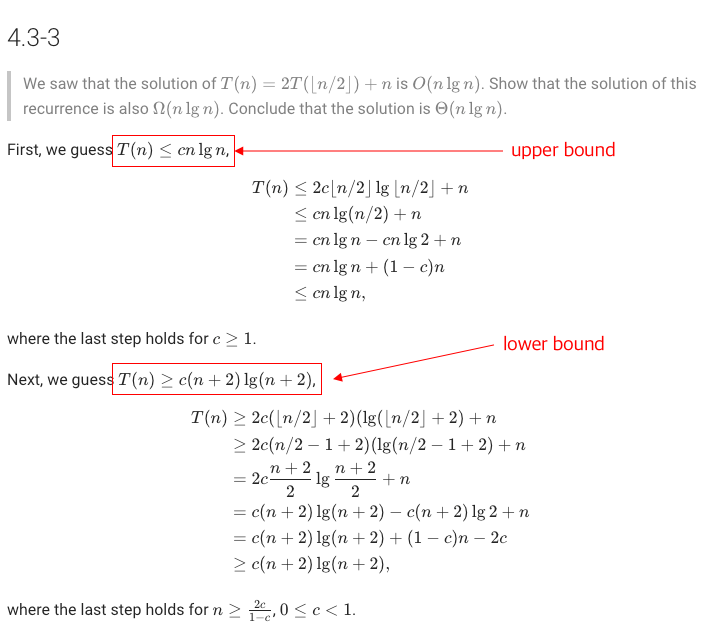
\includegraphics[width=0.7\linewidth]{images/worksheet_0_solution_1.png}
        \end{center}
    \end{itemize}

    \item
    \setcounter{equation}{0}
    \underline{Recurrence (Merge sort):}

    \begin{align*}
        T(n) =
        \begin{cases}
          \Theta(1) & \text{if $n = 1$}\\
          T(\lceil n/2 \rceil) + T(\lfloor n/2 \rfloor) + \Theta(n) & \text{if $n > 1$}
        \end{cases}
    \end{align*}

    \bigskip

    \underline{Guess (upper bound):} $T(n) \leq c \cdot (n-2) \cdot \lg (n-2)$

    \bigskip

    \begin{align}
        T(n) &\leq c(\lceil n/2 \rceil - 2) \lg (\lceil n/2 \rceil - 2) + c (\lfloor n/2 \rfloor - 2)\lg(\lfloor n/2 \rfloor - 2) + dn\\
        &= c(n/2 + 1 - 2) \lg (n/2 + 1 - 2) + c (n/2 + 1 - 2)\lg(n/2 + 1 - 2) + dn\\
        &= c((n-2)/2) \lg ((n-2)/2) + c ((n-2)/2)\lg((n-2)/2) + dn\\
        &= c(n-2) \lg ((n-2)/2) + dn\\
        &= c(n-2) \lg (n-2) - c(n-2) + dn\\
        &= c(n-2) \lg (n-2) - (d - c)n + 2c\\
        &= c(n-2) \lg (n-2)
    \end{align}

    \bigskip

    The bound holds as long as $c > d$.

    \bigskip

    \underline{Guess (lower bound):} $c \cdot (n-2) \cdot \lg (n-2) \leq T(n)$


    \bigskip

    \begin{align}
        T(n) &\leq c(\lceil n/2 \rceil + 1) \lg (\lceil n/2 \rceil + 1) + c (\lfloor n/2 \rfloor + 1)\lg(\lfloor n/2 \rfloor + 1) + dn\\
        &\leq c(n/2 - 1 + 1) \lg (n/2 - 1 + 1) + c (n/2 - 1 + 1)\lg(n/2 - 1 + 1) + dn\\
        &= c(n/2) \lg (n/2) + c (n/2)\lg(n/2) + dn\\
        &= cn \lg(n/2) + dn\\
        &= cn \lg(n) - cn + dn\\
        &= cn \lg(n) + (d - c)n\\
        &\leq c(n-1) \lg(n-1)
    \end{align}

    \bigskip

    The bound holds as long as $d > c$, and $0 \leq c < 1$

    \bigskip


    \underline{\textbf{Notes:}}

    \bigskip

    \begin{itemize}
        \item the $n$ here is asymptotically large
    \end{itemize}

    \item

    \underline{Recurrence:} $T(n) = 2T(\lfloor n/2 \rfloor + 17) + n$

    \bigskip

    \underline{Guess (upper bound):} $cn \lg n$

    \bigskip

    \begin{align}
        T(n) &\leq 2c(\lfloor n/2 \rfloor + 17)\lg(\lfloor n/2 \rfloor + 17) + n\\
        &\leq 2c((n/2) + 17) \lg ((n/2) + 17) + n\\
        &= 2c(n/2) \lg (n/2) + n\\
        &= cn (\lg(n) - 1) + n\\
        &= cn \lg (n) - cn + n\\
        &\leq cn \lg (n) - cn + cn\\
        &= cn \lg (n)
    \end{align}

    \item
    \setcounter{equation}{0}
    \begin{align}
        T(n) &= 4T(n/3) + n\\
        &\leq 4c (n/3)^{\log_3 4} + n\\
        &\leq 4c(1/3)^{\log_3 4}n^{\log_3 4} + n\\
        &\leq (4/4)cn^{\log_3 4} + n\\
        &\leq cn^{\log_3 4} + n
    \end{align}

    We cannot advance further since $n$ in $cn^{\log_3 4} + n$ cannot be eliminated.

    \bigskip

    With the new guess $T(n) \leq cn^{\log_3 4} - dn$, we have

    \begin{align}
        T(n) &= 4T(n/3) + n\\
        &\leq 4c(n/3)^{\log_3 4} - d(n/3) + n\\
        &= 4c(n/3)^{\log_3 4} - d(n/3) + n\\
        &= (4/3^{\log_3 4})cn^{\log_3 4} - d(n/3) + n\\
        &= (4/4)cn^{\log_3 4} - d(n/3) + n\\
        &= cn^{\log_3 4} - d(n/3) + n\\
        &\leq cn^{\log_3 4} - d(n/3) + n\\
        &\leq cn^{\log_3 4}
    \end{align}

    \bigskip

    The bound holds as long as $d \geq 3$ and $c \geq 1$.

    \bigskip

    \begin{mdframed}
        \underline{\textbf{Correct Solution:}}

        \underline{Recurrence:} $T(n) = 2T(\lfloor n/2 \rfloor + 17) + n$

        \bigskip

        \underline{Guess (upper bound):} $cn \lg n$

        \bigskip

        \begin{align}
            T(n) &\leq 2c(\lfloor n/2 \rfloor + 17)\lg(\lfloor n/2 \rfloor + 17) + n\\
            &\leq 2c((n/2) + 17) \lg ((n/2) + 17) + n\\
            &= 2c(n/2) \lg (n/2) + n\\
            &= cn (\lg(n) - 1) + n\\
            &= cn \lg (n) - cn + n\\
            &\leq cn \lg (n) - cn + cn\\
            &= cn \lg (n)
        \end{align}

        \item
        \setcounter{equation}{0}
        \begin{align}
            T(n) &= 4T(n/3) + n\\
            &\leq 4c (n/3)^{\log_3 4} + n\\
            &\leq 4c(1/3)^{\log_3 4}n^{\log_3 4} + n\\
            &\leq (4/4)cn^{\log_3 4} + n\\
            &\leq cn^{\log_3 4} + n
        \end{align}

        We cannot advance further since $n$ in $cn^{\log_3 4} + n$ cannot be eliminated.

        \bigskip

        With the new guess $T(n) \leq cn^{\log_3 4} - dn$, we have

        \begin{align}
            T(n) &= 4T(n/3) + n\\
            &\leq 4c(n/3)^{\log_3 4} - \color{red}4d(n/3)4d(n/3) + n\\
            &\color{red}= 4d(n/3)= 4c(n/3)^{\log_3 4} -4 d(n/3) + n\\
            &\color{red}= 4d(n/3)= (4/3^{\log_3 4})cn^{\log_3 4} - 4d(n/3) + n\\
            &\color{red}= (4/4)cn^{\log_3 4} - 4d(n/3) + n\\
            &\color{red}= cn^{\log_3 4} - 4d(n/3) + n\\
            &\color{red}\leq cn^{\log_3 4} - 4d(n/3) + n\\
            &\color{red}\leq cn^{\log_3 4} - 4d(n/2) + n\\
            &\color{red}\leq cn^{\log_3 4} - 2dn + n\\
            &\color{red}\leq cn^{\log_3 4} - 2dn + dn\\
            &\color{red}\leq cn^{\log_3 4} - dn
        \end{align}

        \bigskip

    \end{mdframed}

    \item I need to show $T(n) \leq cn^2$

    \bigskip

    \begin{align}
        T(n) &= 4T(n/2) + n\\
        &\leq 4c(n/2)^2 + n\\
        &= (4/4)cn^2 + n\\
        &= cn^2 + n
    \end{align}

    \bigskip

    We cannot advance further since $n$ in $cn^2 + n$ cannot be eliminated.

    \bigskip

    But with the new guess $T(n) \leq cn^2 - dn$, we have

    \begin{align}
        T(n) &= 4T(n/2) + n\\
        &\leq 4c(n/2)^2 - 4d(n/2) + n\\
        &= (4/4)cn^2 - 2dn + n\\
        &\leq cn^2 - 2dn + dn\\
        &= cn^2 - dn
    \end{align}

    \bigskip

    The bound holds as long as $d \geq 1$ and $c \geq 1$.

    \item
    \setcounter{equation}{0}

    \bigskip

    \underline{\textbf{Solution:}}

    \bigskip

    \begin{center}
    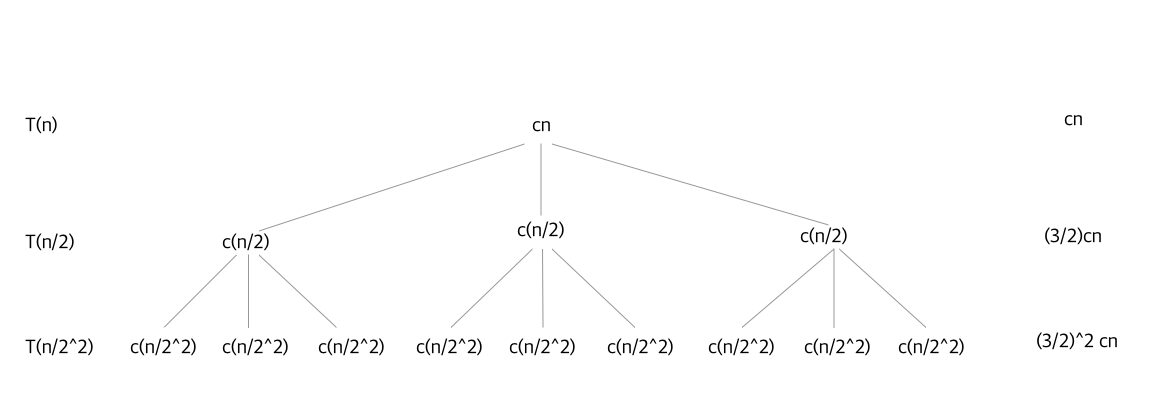
\includegraphics[width=\linewidth]{images/worksheet_0_solution_4.png}
    \end{center}

    \bigskip

    \begin{enumerate}[1.]

        \item Finding number of levels in recursion tree

        \begin{align}
            1 &= n/2^i\\
            2^i &= n\\
            i &= \log_2 n
        \end{align}

        \item Finding the total cost of recursion tree

        \bigskip

        The tree has $n^{\lg 3}$ leaves. So, we have

        \bigskip

        \begin{align}
            T(n) &= n \cdot \sum\limits_{i=0}^{\lg_2(n) - 1} (3/2)^i + \Theta(n^{\lg 3})\\
            &= n \cdot \Bigl( \frac{(3/2)^{\lg_2(n)} - 1}{(3/2) - 1} \Bigr) + \Theta(n^{\lg 3})\\
            &= 2n \cdot \Bigl((3/2)^{\lg_2(n)} - 1 \Bigr) + \Theta(n^{\lg 3})\\
            &= 2n \cdot \Bigl(n^{\lg (3/2)} - 1 \Bigr) + \Theta(n^{\lg 3})\\
            &= 2n \cdot \Bigl(n^{\lg (3/2)} - 1 \Bigr) + \Theta(n^{\lg 3})\\
            &= 2 \cdot \Bigl(n^{\lg 3 - 1 + 1} - n \Bigr) + \Theta(n^{\lg 3})\\
            &= 2 \cdot \Bigl(n^{\lg 3} - n \Bigr) + \Theta(n^{\lg 3})\\
            &= 2 \cdot \Bigl(n^{\lg 3} - n \Bigr) + \Theta(n^{\lg 3})
        \end{align}

        \bigskip

        Thus, the guess for the upper bound is $T(n) = \mathcal{O}(n^{\lg 3})$

        \bigskip

        \item Verifying the correct guess using the subtitution method

        \bigskip

        \underline{Guess:} $T(n) \leq cn^{\lg 3} - dn$

        \bigskip

        I need to show the guess holds in the recurrence $T(n) = 3T(\lfloor n/2 \rfloor) + n$.

        \bigskip

        Indeed we have

        \begin{align}
            T(n) &= 3T(\lfloor n/2 \rfloor) + n \\
            &\leq 3(c \lfloor n/2 \rfloor^{\lg 3}) - d(\lfloor n/2 \rfloor) + n\\
            &= 3\Bigl(\frac{cn^{\lg 3}}{3} - d(\frac{n}{2} + 1) \Bigr) + n\\
            &= 3\Bigl(\frac{cn^{\lg 3}}{3} - \frac{3dn}{2} \Bigr) + n\\
            &\leq 3\Bigl(\frac{cn^{\lg 3}}{3} - \frac{3dn}{3} \Bigr) + n\\
            &= cn^{\lg 3} - 3dn + n\\
            &\leq cn^{\lg 3} - 3dn + 2dn\\
            &= cn^{\lg 3} - dn
        \end{align}

        \bigskip

        And the boundary holds as long as $c \geq 0$ and $d \geq 1$.
    \end{enumerate}

    \bigskip

    \underline{\textbf{Notes:}}

    \bigskip

    \begin{itemize}
        \item Recursion Tree

        \begin{itemize}
            \item Provides a straightforward way to provide a good guess.
            \item Is then verified using subtitution method
        \end{itemize}

        \bigskip

        \underline{\textbf{Example:}}

        \bigskip

        \underline{Recurrence:} $T(n) = 2T(n/2) + 4n, T(1) = 4$

        \bigskip


        \begin{center}
        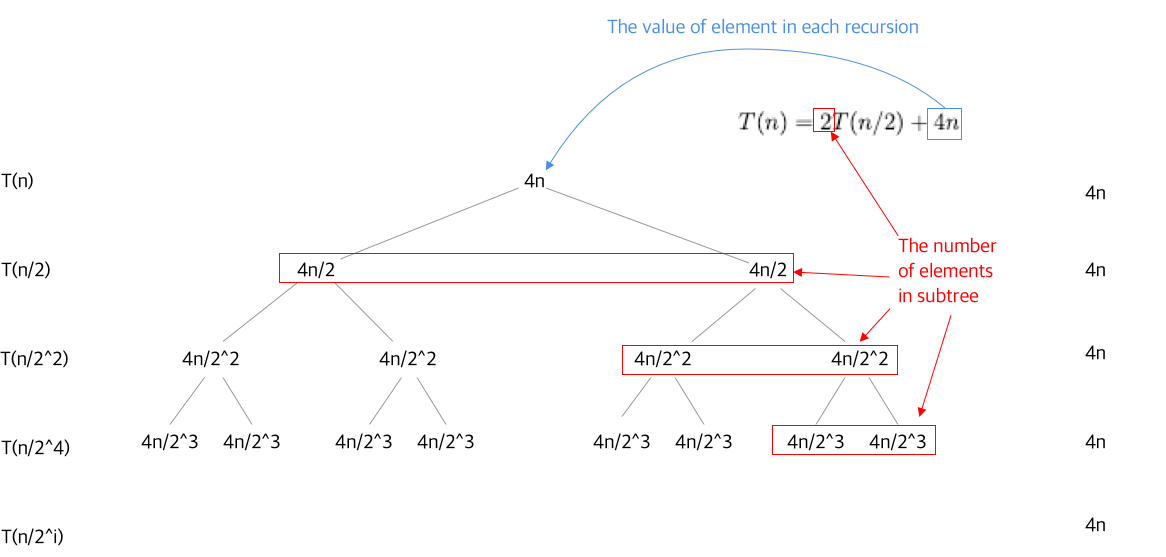
\includegraphics[width=\linewidth]{images/worksheet_0_solution_2.png}
        \end{center}

        \begin{enumerate}[1.]
            \item Finding number of levels in recursion tree

            \begin{align}
                1 &= n/2^i\\
                2^i &= n\\
                i &= \log_2 n
            \end{align}

            \item Finding the value of guess

            \begin{align}
            \sum\limits_{i=0}^{\log_2 n} 4n &= 4n \cdot \sum\limits_{i=0}^{\log_2 n} 1\\
            &= 4n (\log_2 n + 1)
            \end{align}
        \end{enumerate}

        \bigskip

        \underline{\textbf{Example 2:}}

        \bigskip

        \underline{Recurrence:} $T(n) = 3T(n/4) + cn^2$

        \bigskip

        \begin{center}
        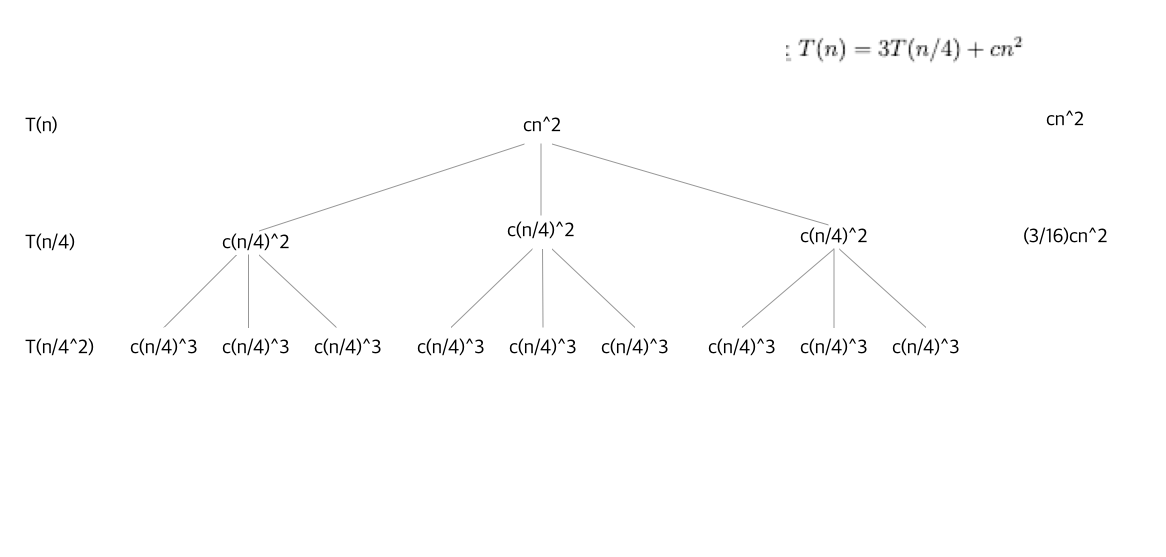
\includegraphics[width=\linewidth]{images/worksheet_0_solution_3.png}
        \end{center}

        \bigskip

        \underline{Steps:}

        \bigskip

        \begin{enumerate}[1.]
            \item Finding number of levels in recursion tree

            \begin{align}
                1 &= n/4^i\\
                4^i &= n\\
                i &= \log_4 n
            \end{align}

            \item Finding the cost of entire tree

            \begin{align}
            T(n) &= \sum\limits_{i=0}^{\log_4 n - 1} c(3/16)^in^2 + \Theta(n^{\log_4 3})\\
            &= cn^2 \cdot \sum\limits_{i=0}^{\log_4 n - 1} (3/16)^i + \Theta(n^{\log_4 3})\\
            &< cn^2 \cdot \sum\limits_{i=0}^{\infty} (3/16)^i + \Theta(n^{\log_4 3}) & [\text{since $n$ is asympt. large}]\\
            &= cn^2 \Bigl(\frac{1}{1 - (3/16)} \Bigr) + \Theta(n^{\log_4 3}) & [\text{Since $\sum\limits_{i=0}^{\infty} ar^i = \frac{a}{1 - r}$}]
            \end{align}

            \bigskip

            \begin{itemize}
                \item \textbf{Note:} $(\log_4 (n - 1)$ because in $i = 0, ... i = \log_4 (n - 1)$ there are $\log_4 (n)$ elements
            \end{itemize}


            \item Finding the upper bound of $T(n)$

            \bigskip

            Since the total cost is $ T(n) = cn^2 \Bigl(\frac{1}{1 - (3/16)} \Bigr) + \Theta(n^{\log_4 3})$,
            we have $\mathcal{O}(n^2)$

            \bigskip

            \item Verify the correctness of guess using subtitution method

            \bigskip

            \begin{align}
                T(n) &\leq 3T(\lfloor n/4 \rfloor) + cn^2\\
                &\leq 3d \lfloor n/4 \rfloor^2 + cn^2\\
                &\leq 3d (n/4)^2 + cn^2\\
                &= (3/16) dn^2 + cn^2\\
                &\leq dn^2
            \end{align}

            \bigskip

            where the last step holds as long as $d \geq (16/13)c$.
        \end{enumerate}


    \end{itemize}

    \item

    \setcounter{equation}{0}

    \bigskip

    \underline{\textbf{Solution:}}

    \bigskip

    \begin{center}
    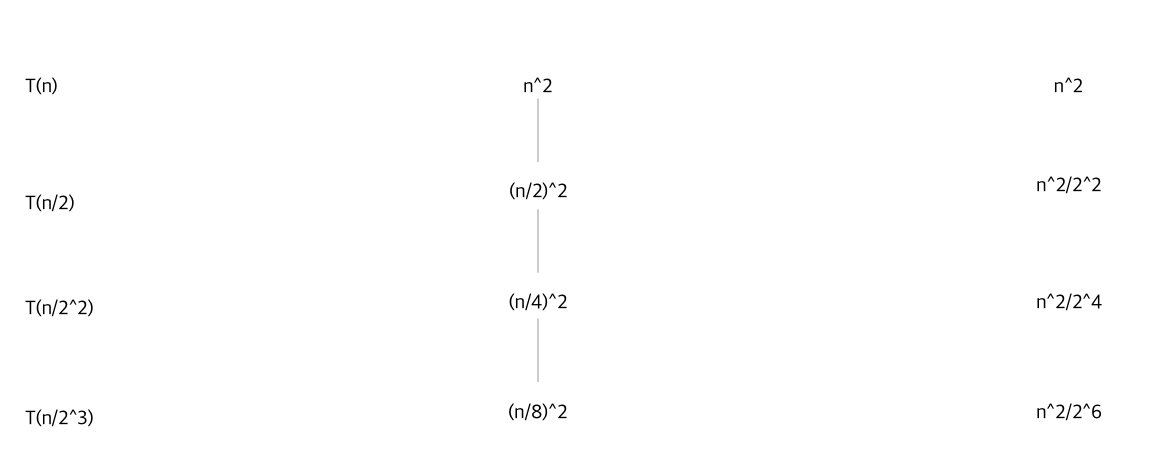
\includegraphics[width=\linewidth]{images/worksheet_0_solution_5.png}
    \end{center}

    \begin{enumerate}[1.]
        \item Finding number of levels in recursion tree

        \begin{align}
            1 &= \frac{n}{2^i}\\
            2^i &= n\\
            i &= \lg n
        \end{align}


        \item Finding the upper bound of $T(n)$

        \begin{align}
            T(n) &= n^2 \cdot \sum\limits_{i=0}^{\lg n - 1} \frac{1}{2^{2i}} + \Theta(1)\\
            &= n^2 \cdot \sum\limits_{i=0}^{\infty} \frac{1}{2^{2i}} + \Theta(1) & [\text{since $n$ is asympt. large}]\\
            &= n^2 \cdot \Bigl ( \frac{1}{1 - \frac{1}{4}} \Bigr) + \Theta(1)\\
            &= \frac{4n^2}{3} + \Theta(1)
        \end{align}

        \bigskip

        Thus, we we can conclude $T(n) = \mathcal{O}(n^2)$

        \bigskip


        \item Verify the correctness of guess using subtitution method

        \bigskip

        \underline{Guess:} $T(n) \leq cn^2$

        \bigskip

        I need to show the guess holds for the recurrence $T(n) = T(\frac{n}{2}) + n$.

        \bigskip

        And, indeed we have

        \begin{align}
            T(n) &= T(\frac{n}{2}) + n^2\\
            &\leq \frac{cn^2}{4} + n^2\\
            &=  (\frac{c}{4} + 1) \cdot n^2\\
            &\leq cn^2
        \end{align}

        \bigskip

        THe boundary holds when $c \geq \frac{4}{3}$.

    \end{enumerate}

    \item
    \setcounter{equation}{0}
    \underline{\textbf{Solution:}}

    \bigskip

    \begin{center}
    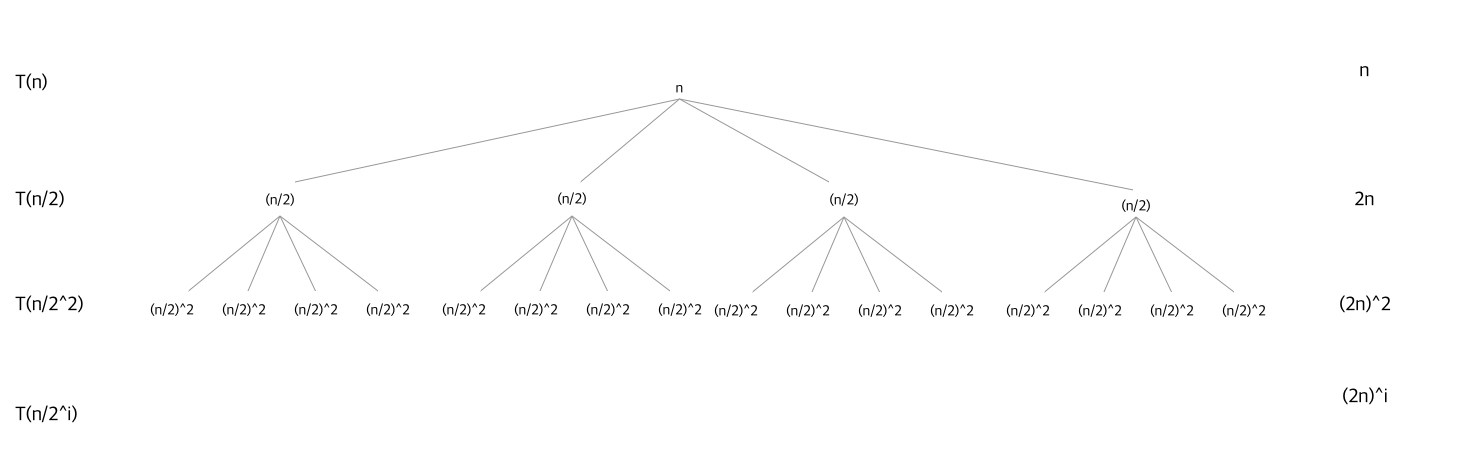
\includegraphics[width=\linewidth]{images/worksheet_0_solution_6.png}
    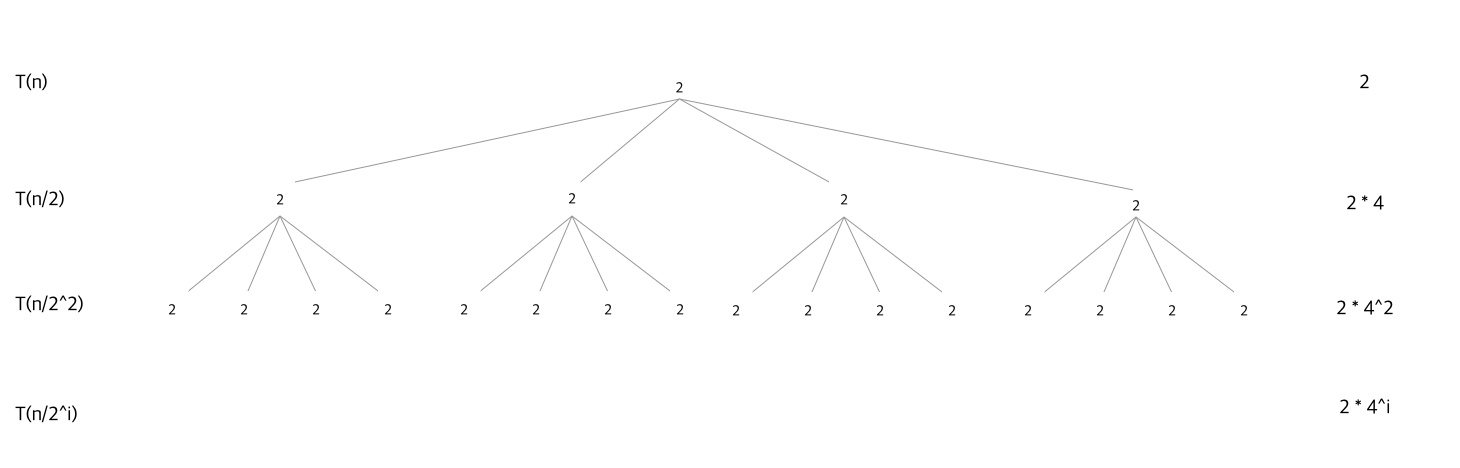
\includegraphics[width=\linewidth]{images/worksheet_0_solution_7.png}
    \end{center}

    \begin{itemize}
        \item Find the total cost of the recursion tree

        \begin{align}
            1 &= \frac{n}{2^i}\\
            2^i &= n\\
            i &= \lg n
        \end{align}

        \item Finding the upper bound of $T(n)$

        \begin{align}
            T(n) &=  \sum\limits_{i=0}^{\lg n - 1} (2 \cdot 4^i + n2^i) + \Theta(n^2)\\
            &= \sum\limits_{i=0}^{\lg n - 1} 2 \cdot 4^i + \sum\limits_{i=0}^{\lg n - 1} n2^i + \Theta(n^2)\\
            &= 2 \cdot \sum\limits_{i=0}^{\lg n - 1} 4^i + n \cdot \sum\limits_{i=0}^{\lg n - 1} 2^i + \Theta(n^2)\\
            &= 2 \cdot \Bigl( \frac{4^{\lg n} - 1}{4 - 1} \Bigr) + n \cdot ( n - 1) + \Theta(n^2) & [\text{Since $\sum\limits_{i=0}^{n-1} ar^i = a \cdot \frac{r^n - 1}{r - 1}$, where $r \neq 1$}]\\
            &= \frac{2}{3} \cdot ( n^2 - 1)+ n \cdot (n - 1) + \Theta(n^2)\\
            &= \mathcal{O}(n^2) + \Theta(n^2)\\
        \end{align}

        \item Verify the correctness of guess using subtitution method

        \bigskip

        \underline{Guess:} $T(n) \leq cn^2 - dn$.

        \bigskip

        I need to show the guess holds for the recurrence $T(n) = 4T(\frac{n}{2} +2) + n$

        \bigskip

        \begin{align}
            T(n) &= 4T(\frac{n}{2} +2) + n\\
            &\leq 4c (\frac{n}{2} + 2)^2 - 4dn  + n\\
            &= 4c (\frac{n^2}{4} + 2n + 4) - 4dn  + n\\
            &\leq cn^2 - 4dn  + n & [\text{Since $n^2$ dominates $n$ asymptotically}]\\
            &\leq cn^2 - 4dn  + 3dn\\
            &= cn^2 - dn
        \end{align}

    \end{itemize}

    \bigskip

    \begin{mdframed}
        \underline{\textbf{Correct Solution:}}

        \begin{center}
            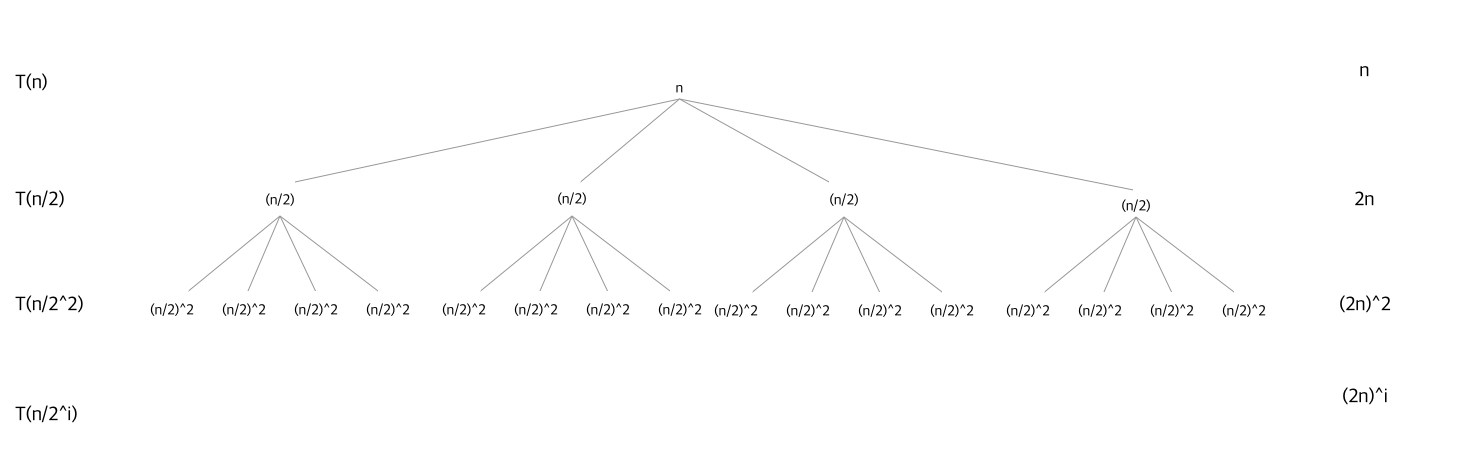
\includegraphics[width=\linewidth]{images/worksheet_0_solution_6.png}
            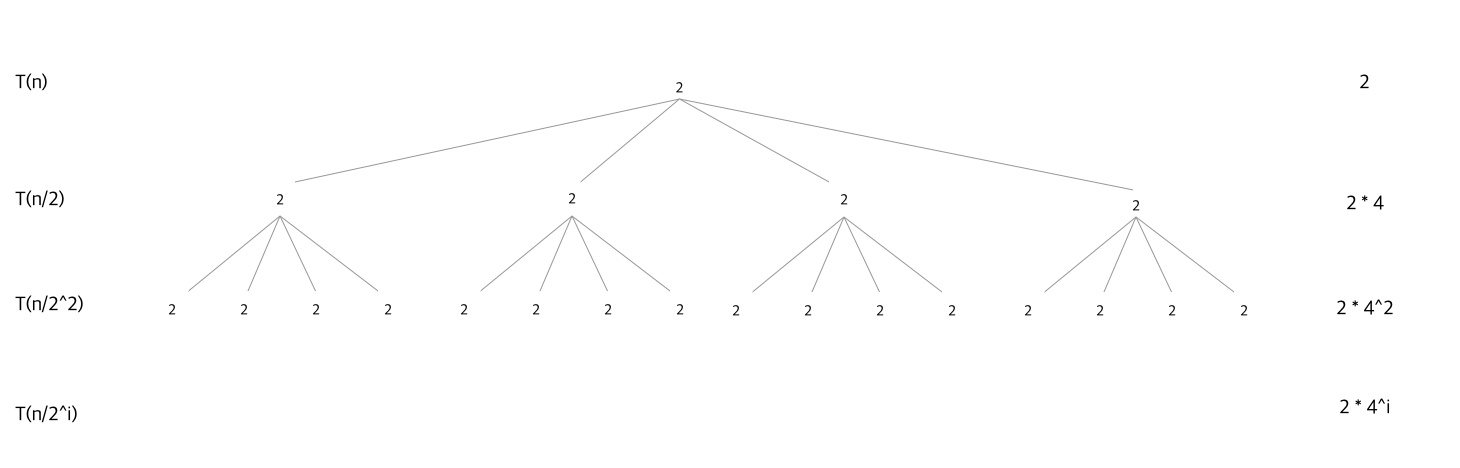
\includegraphics[width=\linewidth]{images/worksheet_0_solution_7.png}
            \end{center}

            \begin{itemize}
                \item Find the total cost of the recursion tree

                \begin{align}
                    1 &= \frac{n}{2^i}\\
                    2^i &= n\\
                    i &= \lg n
                \end{align}

                \item Finding the upper bound of $T(n)$

                \begin{align}
                    T(n) &=  \sum\limits_{i=0}^{\lg n - 1} (2 \cdot 4^i + n2^i) + \Theta(n^2)\\
                    &= \sum\limits_{i=0}^{\lg n - 1} 2 \cdot 4^i + \sum\limits_{i=0}^{\lg n - 1} n2^i + \Theta(n^2)\\
                    &= 2 \cdot \sum\limits_{i=0}^{\lg n - 1} 4^i + n \cdot \sum\limits_{i=0}^{\lg n - 1} 2^i + \Theta(n^2)\\
                    &= 2 \cdot \Bigl( \frac{4^{\lg n} - 1}{4 - 1} \Bigr) + n \cdot ( n - 1) + \Theta(n^2) & [\text{Since $\sum\limits_{i=0}^{n-1} ar^i = a \cdot \frac{r^n - 1}{r - 1}$, where $r \neq 1$}]\\
                    &= \frac{2}{3} \cdot ( n^2 - 1)+ n \cdot (n - 1) + \Theta(n^2)\\
                    &= \color{red}\Theta(n^2)\color{black}
                \end{align}

                \item Verify the correctness of guess using subtitution method

                \bigskip

                \underline{Guess:} $T(n) \leq cn^2 - dn$.

                \bigskip

                I need to show the guess holds for the recurrence $T(n) = 4T(\frac{n}{2} +2) + n$

                \bigskip

                \begin{align}
                    T(n) &= 4T(\frac{n}{2} +2) + n\\
                    &\leq 4c (\frac{n}{2} + 2)^2 - 4dn  + n\\
                    &= 4c (\frac{n^2}{4} + 2n + 4) - 4dn  + n\\
                    &\leq cn^2 - 4dn  + n & [\text{Since $n^2$ dominates $n$ asymptotically}]\\
                    &\leq cn^2 - 4dn  + 3dn\\
                    &= cn^2 - dn
                \end{align}

            \end{itemize}
    \end{mdframed}

    \underline{\textbf{Notes:}}

    \bigskip

    \begin{itemize}
        \item The solution has $4^{\lg n} = n^2$. I noticed the same for $3^{\lg n} = n^3$.
        I had trouble looking for relevant formulas. Is this true in general?
        I can I replace variables in powers with the base?
        \item Noticed that in solution, the total cost is found for each term in $T(\frac{n}{2} + 2)$ (i.e. first for $\frac{n}{2}$ and second for $2$).
        and then combined together in the end.
    \end{itemize}

    \item

    \bigskip
    \setcounter{equation}{0}
    \underline{\textbf{Solution:}}

    \bigskip

    \begin{center}
    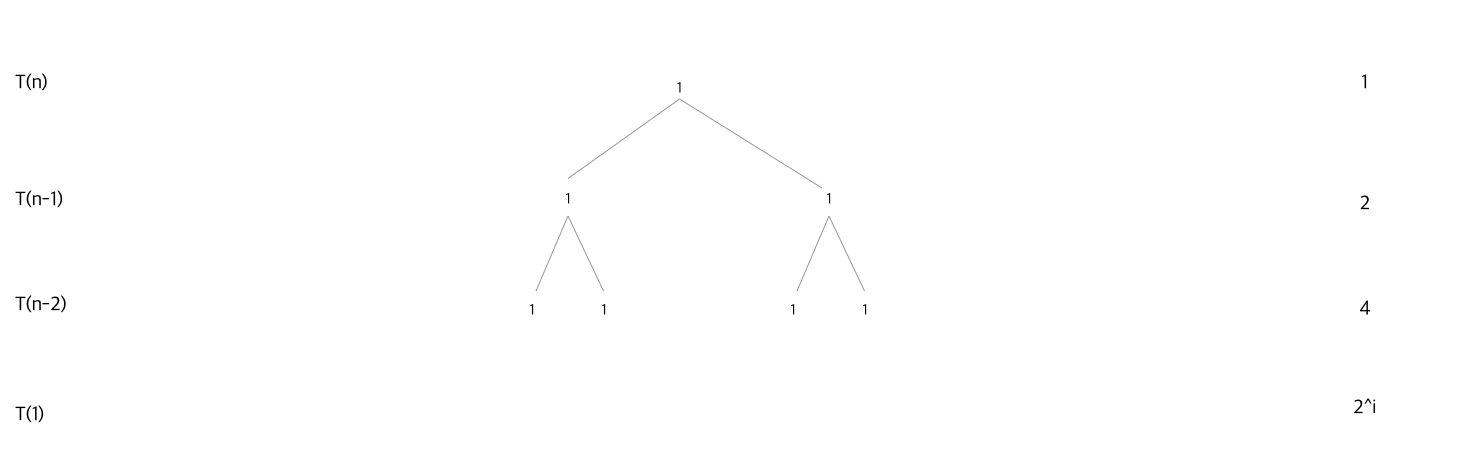
\includegraphics[width=\linewidth]{images/worksheet_0_solution_8.png}
    \end{center}

    \begin{itemize}
        \item Finding the depth of tree

        \begin{align}
            n - 1
        \end{align}

        \bigskip

        \item Finding the number of leaves in the tree

        \begin{align}
            \text{number of branchings}^{\text{depth of tree}} &= 2^{n - 1}
        \end{align}

        \bigskip

        \item Finding the upper bound of $T(n)$

        \begin{align}
            T(n) &\leq \sum\limits_{i=0}^{n-1} 2^i + \Theta(2^n)\\
            &= \Bigl( \frac{2^n - 1}{2 - 1} \Bigr) + \Theta(2^n)\\
            &= (2^n - 1) + \Theta(2^n)\\
            &= \Theta(2^n)
        \end{align}

        \item Verify the correctness of guess using subtitution method

        \bigskip

        \underline{Guess:} $T(n) \geq c2^n$

        \bigskip

        I need to show the bound holds for $T(n) = 2T(n - 1) + 1$.

        \bigskip

        Indeed we have

        \begin{align}
            T(n) &= 2T(n - 1) + 1\\
            &< 2c 2^{n-1} + 1\\
            &= c2^n + 1\\
            &= c2^n & [\text{Since $n$ is asympt. large}]
        \end{align}

        \bigskip

        And the boundary holds when $c \geq 1$.

    \end{itemize}

    \bigskip

    \underline{\textbf{Notes:}}

    \bigskip

    \begin{itemize}
        \item If constant term in $T$ exists, but The term after $T()$ is constant,
        then it's ignored. It is considered when it's in terms of $n$.

        \item Calculating the number of leaves

        \bigskip

        \begin{align}
            \text{number of branchings}^{\text{depth of tree}}
        \end{align}

        \bigskip

        \underline{\textbf{Example:}}

        $2^{n-1}$ (in above example)
    \end{itemize}

    \item

    \bigskip
    \setcounter{equation}{0}
    \underline{\textbf{Solution:}}

    \bigskip

    I will solve only the upper bound for now.

    \bigskip

    \begin{center}
    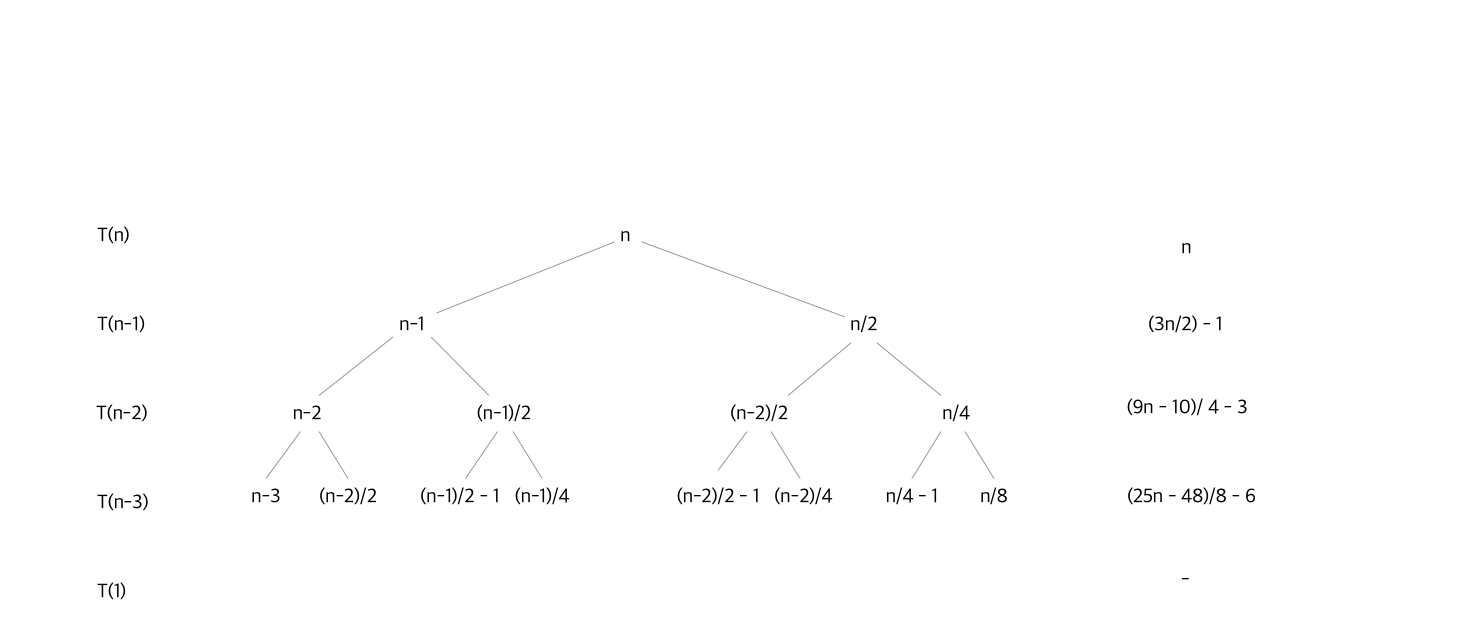
\includegraphics[width=\linewidth]{images/worksheet_0_solution_9.png}
    \end{center}

    \bigskip

    \begin{enumerate}[1.]
        \item Find the depth of longest simple path in recursion tree

        \bigskip

        \quad The longest simple path is created by $T(n-1)$ and has depth of $2^{n-1}$.

        \bigskip

        \item Find the number of leaves expecting a full binary tree of the same depth

        \bigskip

        \quad Here, the number of leaves is at most:

        \begin{align}
            \text{number of branchings}^{\text{depth of tree}} &= 2^{2^{n - 1}}
        \end{align}

        \bigskip

        \item Find the upper bound of $T(n)$ that produces most depth

        \bigskip

        \begin{align}
            \sum\limits_{i=0}^{n-1} 2^i + ... &= \Bigl( \frac{2^n - 1}{2 - 1} \Bigr) + ...\\
            &= (2^n - 1) + ...\\
            &= \mathcal{O}(2^n)
        \end{align}

        \bigskip

        \item Valiate the upper bound using the subtitution method

        \bigskip

        \underline{Guess:} $T(n) \leq c2^{n} - 2dn$

        \bigskip

        I need to show the guess holds for the recurrence $T(n) = T(n-1) + T(\frac{n}{2}) + n$.

        \bigskip

        And indeed we have

        \begin{align}
            T(n) &= T(n-1) + T(\frac{n}{2}) + n\\
            &\leq c2^{n-1} - 2d(n-1) + c2^{\frac{n}{2}} - 2\Bigl(\frac{dn}{2} \Bigr) + n\\
            &= c2^{n-1} - 2d(n-1) + c2^{\frac{n}{2}} - dn + n\\
            &\leq c2^{n-1} - 2d(n-1) + c2^{\frac{n}{2}} - dn + dn\\
            &= c2^{n-1} - 2d(n-1) + c2^{\frac{n}{2}}\\
            &= c2^{n-1} - 2d(n-1) & [\text{Since $c2^{n-1}$ dominates $c2^{\frac{n}{2}}$}]\\
            &= c2^{n} - 2dn & [\text{Since $n$ dominates $-1$}]\\
            &\leq c2^{n} - dn
        \end{align}

        \bigskip

        And the bound holds when $c \geq 1$ (not too sure) and $d \geq 1$.

    \end{enumerate}


    \bigskip

    \underline{\textbf{Notes:}}

    \begin{itemize}
        \item Solving recurrence with uneven recursion tree

        \bigskip

        \underline{\textbf{Example:}} $T(n) = T(\frac{n}{3}) + T(\frac{2n}{3}) + \mathcal{O}(n)$

        \bigskip

        \begin{enumerate}[1.]
            \item Find the depth of longest simple path in recursion tree

            \bigskip

            \color{red}
            The longest simple path is created in $T(\frac{2n}{3})$. With the depth of
            $i = \log_{3/2} n$.
            \color{black}

            \bigskip

            \item Find the number of leaves expecting a full binary tree of the same depth

            \bigskip

            \color{red}
            Here, the number of leaves is $\mathcal{O}(n)$.
            \color{black}

            \bigskip

            \item Find the upper bound of $T(...)$ that produces most depth

            \color{red}

            \begin{align*}
                \mathcal{O}( \text{cost at depth} \times \text{depth}) = \mathcal{O}(cn \log_{3/2} n) = \mathcal{O}(n\lg n)
            \end{align*}

            \color{black}

            \bigskip

            \begin{itemize}
                \item $\mathcal{O}(cn \log_{3/2} n) \to \mathcal{O}(n\lg n)$ since $\frac{3}{2} < 2$ (There seems to be a lot of sloppiness)
            \end{itemize}

            \bigskip

            \item Valiate the upper bound using the subtitution method

            \color{red}
            \begin{align}
                T(n) &\leq T(\frac{n}{3}) + T(\frac{2n}{3}) + cn\\
                &\leq d(\frac{n}{3}) \cdot \lg(\frac{n}{3}) + d(\frac{2n}{3})\lg(\frac{2n}{3}) + cn\\
                &= (d(\frac{n}{3}) \lg n - d(\frac{n}{3}) \cdot \lg 3) + (d (\frac{2n}{3})\lg n - d (\frac{2n}{3})\lg(\frac{3}{2}) + cn)\\
                &= dn \lg n - d( (\frac{n}{3} \lg 3) + (\frac{2n}{3})\lg(3/2) ) + cn\\
                &= dn \lg n - d( (\frac{n}{3}) \lg 3 + (\frac{2n}{3})\lg(3) - (\frac{2n}{3})\lg(2) ) + cn\\
                &= dn \lg n - dn (\lg 3 - \frac{2}{3}) + cn\\
                &\leq dn \lg n
            \end{align}

            \bigskip

            And the above is true as long as $d \geq \frac{c}{\lg 3 - \frac{2}{3}}$

            \color{black}
        \end{enumerate}

        \item I don't feel too sure about how to calculate the number of leaf nodes.
    \end{itemize}

    \item

    \bigskip

    The shortest simple path from the root occurs in $T(\frac{n}{3})$ with the value of $i = \log_3 n$.

    \bigskip

    The figure 4.6 tells us each level in the recurrence tree has cost of $cn$.

    \bigskip

    Since the solution to the recurrence is at least the number of levels times the
    cost of each level, the solution is $\Omega(cn \log_3 n) = \Omega(\frac{cn\lg n}{\lg 3}) = \Omega(n\lg n)$.


    \item
    \setcounter{equation}{0}
    \underline{\textbf{Solution:}}

    \bigskip

    \begin{center}
    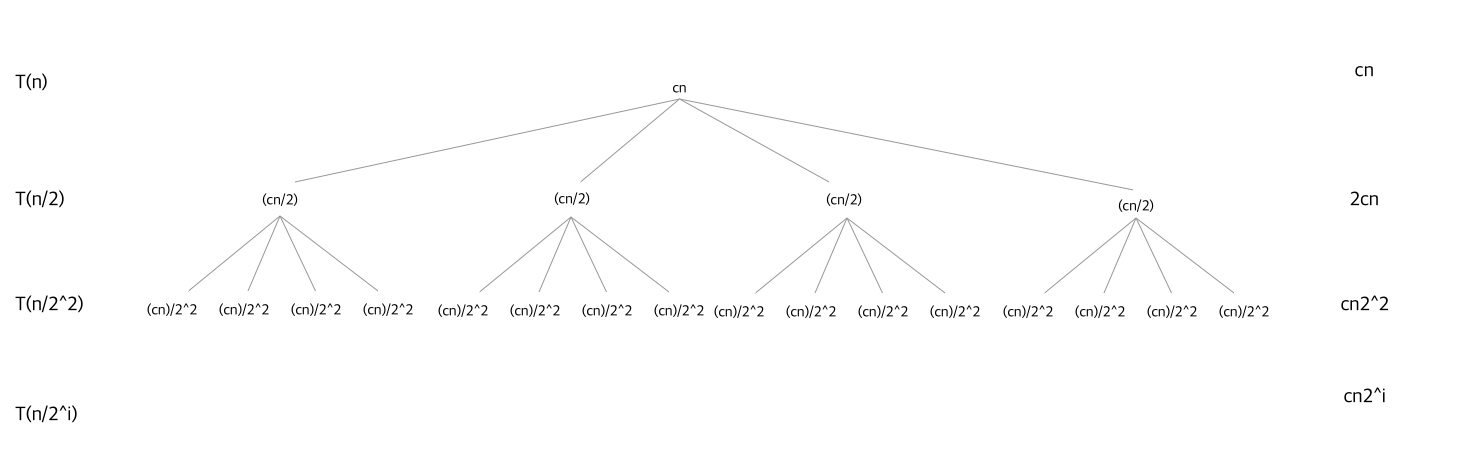
\includegraphics[width=\linewidth]{images/worksheet_0_solution_10.png}
    \end{center}

    \begin{enumerate}[1.]
        \item Finding the depth of tree

        \begin{mdframed}

        The longest simple path from the root to a leaf is $n \to \frac{n}{2} \to \frac{n}{4} \to \cdots \to 1$.

        \bigskip

        Since ($\frac{n}{2^i} = 1$) when $i = \lg n$, the height of the tree is $\lg n$.

        \end{mdframed}

        \item Finding the cost at each level in the tree

        \begin{mdframed}

        Each level has four times more nodes than the level above.

        \bigskip

        So, the number of nodes at depth $i$ is $4^i$.

        \bigskip

        Now, each node at $i = 0, ... , \lg(n) - 1$ has cost of $\frac{cn}{2^i}$.

        \bigskip

        So, by multiplying together, the cost of all nodes at depth $i$ is $cn2^i$

        \end{mdframed}

        \item Finding the cost of leaf nodes

        \begin{mdframed}
        The bottom level, at depth $\lg n$ has $n^{\lg 4} = n^2$ nodes with
        the cost of $n^2T(1)$ or $\Theta(n^2)$.

        \end{mdframed}

        \item Finding the total cost of $T(n)$, or the tight asymptotic bound

        \begin{mdframed}

        \begin{align}
            T(n) &\leq \sum\limits_{i=0}^{\lg n - 1} cn2^i + \Theta(n^2)\\
            &= cn \Bigl( \frac{2^{\lg n} - 1}{2 - 1} \Bigr) + \Theta(n^2)\\
            &= cn(n - 1) + \Theta(n^2)\\
            &= \Theta(n^2)
        \end{align}

        \bigskip

        Thus, the tight asymptotic bound is $\Theta(n^2)$.

        \end{mdframed}

        \item Verifying the upper bound

        \begin{mdframed}

        Let the guess be $T(n) \leq dn^2 - en$.

        \bigskip

        I need to show the guess holds for the recurrence $T(n) = 4T(\lfloor n/2 \rfloor) + cn$.

        \bigskip

        Indeed we have

        \begin{align}
            T(n) &= 4T(\lfloor n/2 \rfloor) + cn\\
            &\leq 4d\lfloor \frac{n}{2} \rfloor^2 - 4e\lfloor \frac{n}{2} \rfloor + cn\\
            &\leq 4d\Bigl(\frac{n}{2} \Bigr)^2 - 4e\Bigl( \frac{n}{2} - 1 \Bigr) + cn\\
            &= 4d\Bigl(\frac{n^2}{4} \Bigr) - e\Bigl( 2n - 4 \Bigr) + cn\\
            &= dn^2 - e\Bigl( 2n - 4 \Bigr) + cn\\
            &= dn^2 - e\Bigl( 2n - 4 \Bigr) + cn & [\text{since $n$ is asympt. large}]\\
            &= dn^2 - e2n + cn\\
            &= dn^2 - n(e2 - c)\\
            &\leq dn^2 - ne
        \end{align}

        \bigskip

        as long as $c \geq e$ and $d \geq 1$.

        \end{mdframed}

        \item Verifying the lower bound

        \bigskip

        \begin{mdframed}

        Let the guess be $d(n+2)^2 \leq T(n)$.

        \bigskip

        I need to show the guess holds for the recurrence $T(n) = 4T(\lfloor n/2 \rfloor) + cn$.

        \bigskip

        Indeed we have

        \begin{align}
            T(n) &= 4T(\lfloor n/2 \rfloor) + cn\\
            &\geq 4d (\lfloor \frac{n}{2} \rfloor + 2)^2 + cn\\
            &\geq 4d (\frac{n}{2} - 1 + 2)^2 + cn\\
            &= 4d \Bigl( \frac{n}{2} + 1 \Bigr)^2 + cn\\
            &= d \Bigl( n + 2 \Bigr)^2 + cn\\
            &\geq d(n+2)^2
        \end{align}

        \bigskip

        as long as $c \geq 0$ and $d \geq 1$.

        \end{mdframed}

    \end{enumerate}

    \item
    \setcounter{equation}{0}
    \bigskip

    \underline{\textbf{Notes:}}

    \bigskip

    \begin{itemize}
        \item Master method

        \begin{itemize}
            \item The master method provides a "cookbook" method for solving recurrences of the
            form


            \begin{align}
                T(n) &= aT(\frac{n}{b}) + f(n)
            \end{align}

            where $a \geq 1$ and $b > 1$ are constants and $f(n)$ is asymptotically positive function.

            \item Allows to solve problems without pencil or paper

        \end{itemize}

        \item Master Theorem

        \begin{itemize}
            \item Let $a \geq 1$ and $b > 1$ be constants, let $f(n)$ be a function, and
            let $T(n)$ be defined on the nonnegative integers by the recurrence

            \bigskip

            $T(n) = aT(\frac{n}{b}) + f(n)$

            \bigskip

            where we interpret $\frac{n}{b}$ to be either $\lfloor \frac{n}{b} \rfloor$ or
            $\lceil \frac{n}{b} \rceil$. Then $T(n)$ has the following asymptotic bounds:

            \begin{enumerate}[1.]
                \item if $f(n) = \mathcal{O}(n^{\log_b (a - \epsilon)})$ for some constant $\epsilon > 0$, then $T(n) = \Theta(n^{\log_b a})$.
                \item if $f(n) = \Theta(n^{\log_b a})$, then $T(n) = \Theta(n^{\log_b a}\lg n)$
                \item if $f(n) = \Omega(n^{\log_b a + \epsilon})$ for some constant $\epsilon > 0$ and if
                $af(\frac{n}{b}) \leq cf(n)$ for some constant $c < 1$ and all sufficiently large $n$,
                then $T(n = \Theta(f(n)))$.
            \end{enumerate}

            \bigskip

            \item Comparing $f(n)$ with the function $n^{\log_b a}$, the larger of two functions determine the solution to the recurrence.

            \bigskip

            \underline{\textbf{Example:}}

            \bigskip

            $T(n) = 9T(\frac{n}{3}) + n$

            \bigskip

            Here $a = 9, b = 3, f(n) = n$. Since $f(n) = \mathcal{O}(n^{\log_3 9 - \epsilon})$
            where $\epsilon = 1$, the case 1 of master theorem tells us $T(n) = \Theta(n^2)$.
        \end{itemize}
    \end{itemize}

\end{enumerate}

\end{document}